% !TEX root = diplomarbeit.tex
\chapter{Firmware}
\renewcommand{\kapitelautor}{Autor: Christina Bornberg, Lucas Ullrich}

%%%%%%%%%%%%%%%%%%%%%%%%%%%%%%%%%%%%%%%%%%%%%%%%%%%%%%%%%%%%%%%%%%%%%%%%%%%%%%%
\section{Allgemeine technische Planung}

  \subsection{Konvention}

    \subsubsection{Koordinaten}
    In der Arbeit wird folgende Konvention festgelegt. Die z-Achse ist die Höhe, die y-Achse ist vorwärts und rückwärts und die x-Achse ist Seitwärts.

    % BILD %

  \subsection{Multicopter}
  Multicopter gehören zu der Luftfahrzeuggattung Hubschrauber.
  Sie starten senkrecht und können durch den Antrieb der Rotoren Neigung erzeugen. Durch diese Neigung kann der Hexacopter nach vorne, zurück, nach links und nach rechts fliegen. 

  \subsection{Anwendungsgebiete}
  \begin{itemize}
    \item Anfertigen von hoch aufgelösten Luftbildkarten
    \item Landvermessung
    \item Thermografie
    \item Baudokumentation
    \item Inspektion und Dokumentation von Brücken, Gebäuden, Gräben etc. mittels Foto und Film
    \item Untermauerung von Gutachten durch bildliche Dokumentation von Brand-, Unfall- oder Wildschäden
    \item Bestands- und Inventaraufnahmen im Straßenbau
    \item Katastrophenschutz

  \cite{copterAnwendung}


  \subsubsection{Funktion}
  Ein Multicopter besteht im Normalfall aus folgenden Komponenten:
  Dem Empfängermodul, dem DJI NAZA-M Flightcontroller sowie der Multicopterhardware (Rotoren, Motoren, Gestell und Leistungselektronik). Der Empfänger des Multicopters kann von einem Sender Steuersignale empfangen und aufgrund der empfangenen Steuersignale Soll-Werte für die Motoren berechnen, um den Multicopter auf die entsprechende Höhe bzw. entsprechende Geschwindigkeit in x, y bzw. z Richtung zu bringen. Wobei onboard Neigungs- und Geschwindigkeitsensoren im DJI NAZA-M Modul für einen stabilen Flug sorgen. 

  Funktion Blockschaltbild (Dokument)

  \subsubsection{Multicopter Arten}
  Es gibt verschiedene Arten von Multicoptern. 
  Je nachdem wie viele Rotoren in einer Ebene liegen, setzt sich der Name zusammen.
  Die bekannteste Art ist der Quadrocopter, welcher 4 Rotoren besitzt. Weiters gibt es Hexacopter mit 6 Rotoren und Octocopter mit 8.


  \subsubsection{Konfiguration}
  Grundsätzlich gibt es 2 Arten einen Multicopter zu Programmieren.
  Einerseits die +-Konfiguration, andererseits die x- beziehungsweise H-Konfiguration. Dabei geht es um die Ausrichtung und die damit verbundene Fluglage.

  % BILD mit 4, 6, 8 in + bzw x %

  \subsubsection{Steuerungsarten} % das is schon wo anders begonnen%
  Signale
  Aileron
  Elevator
  Rudder
  Throttle


\subsection{Programmierung}
  
  Zum Programmieren des Mikrocontrollers von Microchip wurde die Programmiersprache C verwendet.
  Um die Sprache zu lernen, wurde ein sogenanntes Bootcamp als Vorbereitung für die weitere Programmierung veranstaltet.

  Das \textbf{Programmierbootcamp}\\ leitet sich vom militärischen Bootcamp ab, in dem Rekruten ihre Grundausbildung absolvieren. Wie der Name annehmen lässt, lernt man in dieser Version die Grundlagen der Programmierung, hier im Zusammenhang mit Microcontrollern. 

  Einfache Programme, wie ein Lauflicht oder Entfernungsmessung über einen Ultraschallsensor, wurden erstellt.
  Nach dem Initialisieren der Pins, wurde das Programm geschrieben, debuggt und getestet. 
  Die Teile wurden als Grundlage für die Hexacopter Firmware genutzt.

  Durch die einfachen Programme, wurde die Entwicklungsumgebung besser kennengelernt. Die Zeit wurde auch für die Erstellung von Flussdiagrammen und das Einrichten von GitHub genutzt.

  \textbf{Codingrules}\\
  Eine weitere wichtige Aufgabe im Bootcamp war das Erstellen von Codingrules, um einheitliche Programmierung zu ermöglichen. 
  Als Vorbild wurd der C STYLE GUIDE von NASA, Stand: AUGUST 1994, verwendet. \cite{NasaCGuide}
  
  \subsection{Tools}

    \begin{itemize}
      \item \textbf{yEd - Graph Editor}\\ \cite{Tool_yed}
      Zum Erstellen der benötigten Flussdiagramme wurde eine Desktop Anwendung namens yEd verwendet.
      \item \textbf{GitHub}\\ \cite{Tool_github}
      Zur Versionsverwaltung des Codes wurde die digitale Ablage GitHub verwendet. Durch diese ist eine gemeinsame Programmierung möglich.
      \item \textbf{MPLAB}\\ \cite{Tool_mplab}
      MPLAB ist eine Integrierte Entwicklungsumgebung von Microchip. In dieser wurde der Mikrocontroller programmiert und anschließend compiliert.
      Weiters hat die Entwicklungsumgebung eine Git Funktion, wodurch die Daten ohne zusätzliches Tool vom Server herunter- beziehungsweise hinaufgeladen werden können. 
    \end{itemize}


  \subsection{Positionierungssystem}

    \subsubsection{Allgemein} \cite{PositionAllg}
    (geklaut)
    Trackingsysteme werden für die Positionierung benötigt.
    Es gibt mehrere Verfahren, um die Position zu bestimmen:
    Laufzeitverfahren (Ultraschall, GPS, optische Kreisel)
    räumliches Scanning / optische Verfahren (outside-in, inside-out)
    Inertialsysteme (mechanische Kreisel/Gyro, Beschleunigungssensoren)
    mechanische Systeme (Gelenkarm, Seilzug, Exoskelett, Abrollen einer Kugelfläche)
    Phasendifferenz
    Direkte Feldmessung (Elektromagnetisch, Erdmagnetfeld, Gravitation)
    hybride Ansätze (Kombinationen, welche genaue, aber langsame Systeme mit schnellen, ungenaueren integrieren).

    \subsubsection{Anwendung} \cite{posAnwendung}
    Indoor Positionierungssysteme werden derzeit vor allem zur Objekterkennung verwendet, im Umweltmonitoring, über das Detektieren von Bränden in Gebäuden, bis hin zum Einsatz in der Logistik, verwendet. Da es sehr viele unterschiedliche Anwendungsgebiete gibt, werden unterschiedliche Methoden verwendet. 

    \subsubsection{Eigenschaften der Positionsbestimmung}

    Ein Positionierungssystem kann verschiedene Arten von Informationsdaten bereitstellen. 

    \textbf{Physische und symbolische Positionierung}\\
    Die physische Positionierung ist eine exakte Position, die zum Beispiel in einem Koordination, meist in 2-D oder 3-D Karten, bestimmt wird. Längen- und Breitengrade spielen dabei eine wichtige Rolle.
    Symbolische Positionierung ist die abstrakte beschreibung eines Ortes, sie wird sprachlich beschrieben, beispielsweise Küche, Garten, Dachboden.
    Eine physikalische Position kann auch symbolisch Beschrieben werden.
    
    \textbf{Relative und absolute Positionierung}\\
    Die absolute Positionierung verwendet Referenzgitter und Koordinaten. Das Paradebeispiel für absolute Ortung ist die Angabe von Längen­ und Breitengrad.   Die darauf aufsetzende Technik, die sich diese Kartographie zu Nutze macht, ist GPS. 
    Die relative Positionierung legt ihre eigenen Rahmen vor, die auf Basisstationen oder definierten Punkten basieren. Hier wird angegeben, wie weit das Objekt entfernt ist.

    \textbf{Genauigkeit}
    Die Genauigkeit gibt an, wie sehr sich gemessene und tatsächliche Position unterscheiden.

    \textbf{Skalierung}
    Hierbei gibt es mehrere Faktoren, beispielsweise die Anzahl der zu trackenden Objekte, die Reichweite und die benötigte Zeit.

    \textbf{Kosten}
    Hier gibt es Kosten im Bereich der Anschaffung des Systems und Kosten während des Betriebs.

    \textbf{Limitierung}
    Unter Limitierung fallen Einschränkungen und Störfaktoren. Manche Systeme haben besondere Ansprüche an ihre Umgebung.

    \subsubsection{Selbst- und fernortende Lokalisierungstechniken}

    Lokalisierungstechniken können weiter als selbstortend oder fernortend (engl. self­positioning/remote­positioning) klassifiziert werden. Beim optischen Tracking werden die beiden Varianten Inside-out und Outside-in genannt.

    % BILD %

    \textbf{Selbstortendes Positionierungssystem}\\
    Der mobile, bewegliche Empfänger bekommt die Daten von verschiedenen Sendern, die sich auf bekannten Positionen befinden. Die Lokalisation des Empfängers wird durch die gemessenen Signale ermittelt. Das Objekt kann sich selbst orten, es ist kein Netzwerk notwendig.

    \textbf{Fernortendes Positionierungssystem}\\
    Mobile, bewegliche Sender mit stationären, unbeweglichem Empfänger. Die Messdaten aller Empfänger werden gesammelt und die Position des Senders wird in der Zentrale berechnet. Hier ist ein Netzwerk notwendig, sämtliche Berechnungen werden durch eine zentrale Instanz ausgeführt.

    \subsubsection{Signalbasierte Verfahren}

    Verfahren zur Positionsbestimmung   

    \begin{itemize}
      \item \textbf{Lateration}\\
      Bei der Lateration wird die Position mit Hilfe der Entfernungsmessung bestimmt.
      Techniken der Lateration sind TOA (time of arrival) und TDOA (time difference of arrival).
      Bei \textbf{TOA}\\ werden in Laufzeit Signale gemessen. Durch die Zeitdifferenz zwischen Sender und Empfänger, kann die Entfernung errechnet werden. Sender und Empfänger müssen dafür synchronisiert werden. Eine einfache Messung kann die Entfernung zwischen Sender und Empfänger messen. Für die Positionierung, werden 3 Basisstationen benötigt. Durch Trilateration kann dann die Position bestimmt werden.
      % BILD %
      \textbf{TDOA}\\ basiert auf der Zeitdifferenzmessung. 
      Die mobile Sation sendet einen Zeitstempel an drei Basisstationen. Durch die Differenz kann die Position ebenfalls mittels Trilateration bestimmt werden. Auch hier ist eine synchronisation erforderlich.
      % BILD %
      \item \textbf{Angulation}\\
      Bei der Angulation wird die Position durch die Bestimmung von Winkeln ermittelt.
      \textbf{AOA}\\ (Angel of Arrival) wird mittels Berechnung des Einfallswinkels auf ein Antennenarray umgesetzt. Bei dieser Technik werden mindestens 2 Basisstationen benötigt. Mit den Einfallswinkeln der empfangenen Signale kann die Position durch Triangulation festgestellt werden. Die Winkelbeziehungen eines Dreiecks werden dafür verwendet.
      Bei dieser Technik muss keine Synchronisation durchgeführt werden. Der Nachteil ist die benötigte komplexe Hardware. 
      % BILD %
      \item \textbf{Scene Analysis}\\
      Bei der Szenenanalyse werden Umgebungsparameter erfasst und ausgewertet.
      \textbf{Fingerprint}\\
      Für diese Technik werden Signalstärken gemessen und als Fingerprint abgespeichert. Die Position wird dann durch den Vergleich von Fingerprints mit der Signalstärke, die bei der aktuellen Position gemessen wird, herausgefunden.
      \item \textbf{Proximity}\\
      Für das Verfahren Proximity wird die physische Nähe genutzt.
      Hier gibt es die Technik COO (cell of origin).
      Bei \textbf{COO}\\ gibt es Basisstationen, mit bekannter Position. Die mobile Station verbindet sich mit der nächstgelegenen Basisistation.Wenn die mobile Station von mehreren Basisstationen erkannt wird, wird die Signalstärke beachtet.
      Diese Methode ist sehr ungenau.
      % BILD %
    \end{itemize}

    \subsubsection{Signalbasierte Technologien}\\
    \begin{itemize}
        \item \textbf{GPS (Global Positioning System)}\\
        GPS ist ein satellitengestützte Navigationssystem, das Ende der 1980er-Jahre zur globalen Positionsbestimmung entwickelt wurde. Die Nachteile des Systems sind der schlechte Empfang der Satellitensignale für indoor- Anwendungen. 
        \item \textbf{RFID (radio-frequency identification)}\\
        RFID bezeichnet eine Technologie für Sender-Empfänger-Systeme zum automatischen und berührungslosen Identifizieren und Lokalisieren von Objekten mit Radiowellen. Ein RFID-System besteht aus einem Transponder, der sich am oder im Objekt befindet und einen kennzeichnenden Code enthält, sowie einem Lesegerät zum Auslesen dieser Kennung. 
        \item \textbf{WPS (WLAN Positioning System)}\\    
        WPS ist ein indoor Positionierungssystem, das auf WLAN basiert. Durch sogenannte  Access Points (de. drahtloser Zugangspunkt), wird die Entfernung zu Endgeräten bestimmt. Durch drei Accesspoints kann mittels Dreiecksmethode, die Position des Endgeräts ermittelt werden.
        \item \textbf{Ultraschall}\\
        Ein Ultraschallsensor ist Sender und Empfänger in einem. Er sendet ein Signal, dieses wird reflektiert und anschließend empfängt der Sensor sein Echo.
        Durch die Information, mit welcher Geschwindigkeit sich elektromagnetische sowie akustische Wellen ausbreiten, ist es möglich Entfernungen zu messen. Die Zeit, die ein Signal zum zu messenden Objekt und wieder zurück braucht, nennt man Laufzeit.
    \end{itemize}

    \subsubsection{Optische Verfahren}
    http://whatis.techtarget.com/definition/machine-vision

    Maschinelles Sehen (machine vision) beschreibt die Fähigkeit eines Computers zu sehen. Anders als das menschliche Auge, können Kameras auch Infrarotlicht, Ultraviolettes Licht und Röngtenstrahlen wahrnehmen. 

    Evtl noch kurz unterschied Mensch & Maschine

    Methoden zur Bildverarbeitung \cite{Bildverarbeitung}

    Segmentierungsmethoden (Aufteilung von Bildern in Bereiche)
      Thresholding: Histogrammbasierte Segmentierung: Konvertierung des Grauwertbildes in ein binäres Bild
        Techniken: statistische und dynamische Schwellenwerte
        Techniken: mit einem oder mehreren Schwellenwerten
      Kantenbasiernde Segmentierung
      Regionenbasierende Segmentierung: Benachbarte Pixel werden auf Gleichheit zum Startpixel geprüft.
    Merkmalextraktion:Durchsuchung eines Bildes nach Kanten, Ecken und Templates
      Kantendetektoren
        Sobel Kantendetektion: Faltung des Bildes mit Hilfe einer Sobel-Matrix und anschließende Approximation der ersten Ableitung des Bildes
        Canny Kantendetektion: Zur Glättung, Einsatz eines zweidimensionalen Gaußfilters und Einsatz von gerichteten Ableitungsoperatoren. Nach der Ausdünnung der Linien, Anwendung einer Hysterese zur Erkennung ob es sich um eine Kante oder um ein Rauschen handelt.
    Eckendetektoren
      Moravec´s Corner Detector: Betrachtung eines kleinen lokalen Bildfensters und Messung der Intensitätsunterschiede beim Verschieben des Fensters. Erkennung von Kanten und Ecken
      Harris Corner Detector: Betrachtung eines lokalen Bildfensters durch Verschiebung in 4 Richtungen durch die Taylor Entwicklung
    Objekterkennung 
      Templatematching: Modellierbare Segmentierung. Es wird mittels vollständiger Suche entschieden, wie gut das vorgegebene Modell (Template) zu einem bestimmten Pixelbereich passt (match)
      Klassifizierung: Vorgang zur Einteilung von Objekten in Klassen und Kategorien. Zum Klassifizieren werden Merkmale wie Form, Kontrast, Segmentgröße, Farbe, Textur usw. herangezogen.
    Verfolgen von Merkmalen über Bildsequenz 
      Kalman-Filter: Ist ein stochastischer Zustandsschätzer mit iterativer Struktur, der in Echtzeitsystemen angewendet wird unter der Annahme von normalverteilten Vorhersagen und Messungen und Vorhersage von Fehlern.
      Optical Flow: Oberflächen erhalten eine Geschwindigkeit und eine Richtung, wobei die Bewegung von einer 3 D Szene in die 2 D Bildebene unter Berechnung eines Bewegungsvektors, der die Bewegung in Bildkoordinaten ausdrückt.
        Merkmalsbasierte Methoden
        Intensitätsbasierte Methoden
          Gradientenbasierte Techniken
          Korrelationsbasierte Techniken
          Filterbasierte Techniken

\subsubsection{Optische Trackingsysteme}

    Die Lokalisierung von sich bewegenden Objekten und Bewegungserfassung

    \textbf{Pixy CMUcam5}\\
    Die Pixy CMUcam5 ist ein optisches Trackingsystem. Das Kameramodul ist in der Lage, Objekte in 7 verschiedenen Farben zu scannen, diese zu speichern und wiederzuerkennen. Daten über die Höhe und die Breite, sowie die x- und y-Position des getrackten Objektes innerhalb des Frames werden ausgegeben. Bei sogenannten Colorcodes, die sich aus zwei oder mehrfarbigen Objekten ergeben, kann die Rotation des Objektes ebenfalls ermittelt werden.
    \cite{Pixy}

    \textbf{Vicon}\\
    Vicon ist ein System, das mit dem Tracking-Verfahren Motion Capture (Bewegungs-Erfassung) arbeitet. 
    Mehrere Kameras werden in einem Raum verteilt. Jede Kamera besitzt einen Infrarotfilter und Infrarot-LEDs. Die Lampen senden infrarotes Licht aus, dieses wird an Markern, die sich auf dem zu trackenden Objekt befinden, reflektiert. Mithilfe einer Software kann dadurch eine dreidimensionale Karte erstellt werden.
    \cite{Vicon}

  \subsection{Konzepte}
  Die verschiedenen Positionierungsarten wurden verwendet, um Konzepte für die Navigation zu entwickeln.

    \subsubsection{Aufgabenstellung}
    Damit der Hexacopter autonom durch den Raum navigieren kann, benötigt er ein Positionierungssystem.

    \subsubsection{Funkbasiertes Tracking}

      \textbf{Tracking mittels Time of Arival}\\

      Mithilfe der Laufzeitmessung können Objekte, die mit einem Empfänger ausgestattet sind, geortet werden. Dafür wird die Zeit die ein Signal vom Sender zum Empfänger benötigt gemessen. Das Signal ist eine elektromagnetische Welle, die sich im Vakuum in Lichtgeschwindigkeit ausbreitet. Die gemessene Laufzeit wird mit der Lichtgeschwindigkeit multipliziert, damit kann die Entfernung berechnet werden. 

      Bei diesem Konzept, soll durch die benützung sogenannter Pseudolites (Gefälschte Sateliten) eine Art lokales GPS erschaffen werden.

      Wir haben 3 Sender, die signale Schicken, der Empfänger ist im Hexacopter.
      Jeder der 3 Pseudolites sendet ein Signal, dadurch werden 3 Distanzen ausgerechnet.
      Aus diesen 3 Distanzen und der bekannten Koordinaten der Pseudolites, wird die augenblickliche Position mittels Trilateration des Hexacopters berechnet.

      Distanz 1 = (x1 - x)^2 + (y1 - y)^2 + (z1 - z)^2
      Distanz 2 = (x2 - x)^2 + (y2 - y)^2 + (z2 - z)^2
      Distanz 3 = (x3 - x)^2 + (y3 - y)^2 + (z3 - z)^2

      Distanz ... ist die durchgeführte Messung
      x1, y1, ... z2, z3 ... sind die staatischen Koordinaten von den Pseudolites 
      x, y, z ... werden durch die Lösung dieses quadratischen Gleichungssystems ermittelt. 
      
      Beim lösen der Gleichung erhält man 2 Schnittpunken. Dies ergibt sich aus der logischen Schlussfolgerung, dass die Oberflächen 3er verschmolzener Kugeln 2 Schnittpunkte haben.
      Wenn die Pseudoliten am Boden anbringt, liegt eine der beiden Lösungen oberhalb und die 2. Lösung unterhalb des Bodens, womit man einfacherweise, die Lösung mit der negativen Z-Koordinate ausschließen kann.

    \subsubsection{Optisches Tracking}
    % Aufgrund der Komplexität einer signalbasierten

      \textbf{Kamerasystem im Raum}\\

      Beim optischen Tracking mit Markern wird mit Kameras gearbeitet, welche aktive (also ein Signal emittierende) oder passive Marker an den zu erfassenden Personen oder Gegenständen verfolgen. 

      Für ein fernortendes Positionierungssystem, werden Kameras in einem Raum verteilt. 
      Sowohl Tische und Kreuzungen als auch der Hexacopter sind mit Markern versehen. Die einzelnen Komponenten werden vom Kamerasystem erfasst und anschließend wird eine Karte erstellt. Diese Karte besitzt, wie ein Koordinatensystem Längen und Breitengrade.

      Der Hexacopter wählt seine Route, die er mittels Position der Kreuzugen und Tische berechnet.

      Durch das Trackingsystem kann die Position des Hexacopters getrackt werden. Somit wird kontrolliert, ob er sich auf der richtigen Route befindet.

      Anhand der Markerbewegungen in den einzelnen Kamerabildern kann mittels Triangulation die Position der Marker in 3D berechnet werden.

      \textbf{Linien}\\
      Bei einem selbstortenden Positionierungssystem sind Sensoren auf dem sich bewegenden Objekt angebracht.
      Der Hexacopter trackt eine Linie, die Kamera ist am Hexacopter befestigt
      Zunächst wurde ein Konzept mit Linien erstellt. Der Hexacopter folgt einer einfarbigen Linie, bis er zu einer Kreuzung kommt, nun ist seine Aufgabe, die nächste Linie zu finden, um seinen Weg zum Ziel zu finden.  

      Vorteile: Der Hexacopter kann die Linie nur schwer verlieren
      Nachteile: Das verwendete Kamerasystem ist nicht in der Lage eine Linie zu tracken.


      \textbf{Farbcode pro Wegabschnitt}\\
      Durch die Verwendung der Pixy CMUCam5 ergibt sich die Möglichkeit, Farbobjekte, die eine oder mehrere Farben haben, zu scannen.

      Bei diesem Konzept bekommt der Mikrocontroller Informationen zu den Farbobjekten pro Wegabschnitt. Vom Start bis zur ersten Kreuzung verwendet er eine Farbinformation, die aus einem Colorcode besteht. Jedes Farbobjekt auf diesem Weg, hat die selben 2 Farben. Durch diese Technik hat der Administrator des Systems weniger Aufwand.

      Version 1: 1 ColorCode pro Wegabschnitt

      Vorteile:
      - (kein Problem, wenn ein Farbobjekt nicht mitgetrackt wird)

      Nachteile:
      - die Korrektur der Rotation ist komplizierter, da zuerst über das Koordinatensystem der Kamera herausgefunden werden muss, welches Farbobjekt am nächesten zu y = 0 ist. 
      - Weiß nicht, ob das Nächste wirklich das Nächste ist oder ein Fehler

      \textbf{Farbcodes variieren}\\
      Das gewählte System wird ebenfalls mittels 2-farbiger Codes umgesetzt.

      Erklärung: Jedes Farbobjekt hat einen ColorCode

      Vorteile:
      keine großartigen Kosten neben Copter und Server
      Rechnung am Hexacopter
      - relative Position kann besser bestimmt werden
      - kennt das Ende des Weges und muss daher nicht herausfinden, wann der Weg zu ende ist und die Landeplattform vor ihm ist

      Nachteile:
      - (Probleme, sollte ein Farbobjekt nicht erkannt werden)
      - Mehr Aufwand bezüglich auflegen der Farbobjekte -> man muss eine Reihenfolge beachten. Dadurch müssen auch mehrere Daten vom Server geschickt werden. => die Farbinformation ist länger, da jedes einzelne Objekt eingetragen werden muss. 



      \textbf{Tracking mittels Infrarot}\\


      Vorteile:
      System funktioniert ebenfalls im Dunkeln.
      Nachteile: 
      Jeder Tisch benötigt einen Stromanschluss.
      Die Wartung ist aufwändiger.
      Komplexer für den Administrator - wo ist welcher Infrarotsender


      \subsubsection{Das gewählte Konzept}

      Das geählte Konzept ist ein optisches Trackingsystem, bei dem die Farbcodes variieren.

      Um die Höhe zu messen wird eine einfache Entfernungsmessung mittels Ultraschallsensor durchgeführt.

      Das System wurde auf die oben genannten Eigenschaften analysiert:

      \textbf{Physische und symbolische Positionierung}\\
      Die Positionierung erfolgt physisch. Durch die Pixy kann die tatsächliche Position ermittelt werden.
      Zum Besseren verständnis, wir die Positionen ebenfalls symbolisch beschrieben. Es werden die Namen Base, für die Küche beziehungsweise den Stützpunkt, Weg für die Route aus Colorcodes und Tisch, für die Landeplattform, auf der der Hexacopter landen soll, verwendet.

      \textbf{Relative Positionierung}\\
      Das gewählte System gestaltet sich relativ, da der Hexacopter seine Position relativ zu Farbobjekten bestimmt.

      \textbf{Genauigkeit}\\
      Da das System mittels optischem Tracking umgesetzt wird, ist die Genauigkeit sehr hoch.
      
      \textbf{Skalierung}\\

      Das System ist beliebig Skalierbar, da es auf Farbcodes basiert. Es besteht die Möglichkeit, beliebig viele Farbcodes dem Weg hinzuzufügen oder wieder wegzunehmen. Die Routen sind im Adminbereich hinterlegt und müssen, je nach dem, wie der Administrator die Farbcodes legt, diese auch mitverändern. Im System gibt es aus Testgründen eine Grenze von 20 Farbcodes, diese kann aber einfach verändert werden.

      Die Pixy CMUcam5 ist in der Lage 135 Objekte pro Frame zu tracken. Unser System ist selbstortend, dewegen interessiert sich der Hexacopter nur für ein Objekt pro Frame. \cite{PIXY_Porting_Examplecode}

      Das System ist, wegen des Ultraschallsensors auf eine Höhe von 3 Metern begrenzt. Im System ist eine Maximalhöhe von 220m über dem Boden und 120m über einem Tisch hinterlegt.

      \textbf{Kosten}\\
      Da  die Positionierung auf einer Kamera mit Farbcodes, einem Ultraschallsensor, einem Mikcrocontroller und einem WLAN fähigen Gerät basiert, beschränken sich die Kosten auf wenige Hundert Euro

      \textbf{Limitierung}\\
      Die Pixy CMUcam5 muss zuvor gespeicherte Farben wiedererkennen, die Lichtverhältnisse müssen daher optimal sein.  
      Objekte müssen eine Mindestensgröße von 4x1 Pixel in einem Frame ausmachen. Die Pixycam kann Objeke, laut Angaben der Website, über Kilometer tracken, wenn diese groß genug sind. Beispielsweise kann ein Objekt in Ping-Pong Ball Größe aus einer Entfernung von etwa 3 Metern gescannt werden. 
      \cite{Pixy}

      Das System kann sowohl Indoor als auch Outdoor angewendet werden.

      Der verwendete Ultraschallsensor misst die Entfernung mit einer Auflösung von 3mm. Er eignet sich für den Bereich zwischen 2cm und 3m. 
      \cite{Ultrasonic}

      \textbf{Selbstortendes Positionierungssystem}\\
      Das Positionierungssystem ist selbstortend. Die am boden liegenden Farbobjekte werden von der Pixy getrackt und die daraus entstehenden Daten verarbeitet. Der Hexacopter kann ohne externe Einflüsse navigieren und ist somit unabhängig.


  \subsection{Tischkonzept}

  Das Konzept Tischplan beschreibt den Aufbau / die Infrastruktur des Restaurants. Welche Komponenten benötigt werden und wo diese platziert sind.
  Um eine vorgegeben Route fliegen zu können muss der Multicopter einen Routenplan vorgegeben bekommen, in diesem sind die einzelnen Markierungspunkte enthalten, welche der Multicopter auf seinem Weg zum Tisch überfliegt.

  Komponenten des Restaurants, hier kommt die symbolische Positionierung zum Einsatz.

  \textbf{Küche}\\
  Die Küche beschreibt den Bereich, in dem der Kellner interagiert. Hier befindet sich eine Base, dies ist eine Plattform, die mit einem Farbcode ausgestattet ist. Auf ihr steht der Hexacopter und wartet auf die Beladung des auszuliefernden Cupcakes und den Befehl, loszufliegen.
  Das Admin Interface und der Server stehen ebenfalls in der Küche, über diese Komponenten bekommt der Hexacopter Befehle. Die Routen sind im Admin Interface hinterlegt.

  \textbf{Weg}\\
  Der Weg besteht aus sich abwechselnden 2 farbigen Codes. Die Teile zwischen Tischen und Kreuzungen, werden als Wegabschnitt bezeichnet. 

  \textbf{Tisch}\\
  Auf einem Tisch befindet sich, wie in der Küche eine Plattform, die mit einem Farbcode versehen ist. Hier landet der Hexacopter, wartet 30 Sekunden lang und fliegt danach den Weg zurück zu seiner Base. In den 30 Sekunden soll der Cupcake entnommen werden. Weiters befindet sich ein iPad auf jedem Tisch. Durch dieses enthält jeder Tisch seine eigene ID und dazugehörige Route. Bestellungen können somit einem Tisch zugewiesen werden.

  % Bild vom Ablauf %%%%%%%%%%%%%%%%%%%%%%%%%%%%%%%%


  \subsection{Flussdiagramme}
  Für einen besseren Überblick über die einzelnen Programme und deren geforderten Funktionen wurden einzelne Flussdiagramme des gesamten Prozesses erstellt.
  Diese dienen nachfolgend als Orientierung beim Programmieren der einzelnen Funktionen.

  \begin{figure}[tbh]
    \begin{centering}
      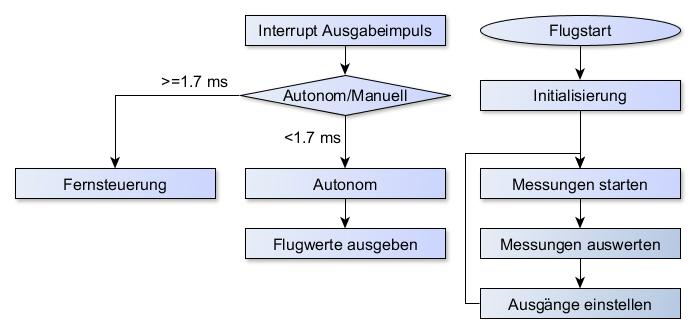
\includegraphics[width = \textwidth]{Bilder/Flussdiagramm}
    \par\end{centering}
    \caption{Flussdiagramm des Gesamtablaufs}
    \label{Flussdiragramm}
  \end{figure}

  Für die weiteren Programmteile wurden jeweils noch detailliertere Flussdiagramme erstellt.

  \subsection{Aufbau des Programms}

  % Erklärung, wer was Aufruft %





%%%%%%%%%%%%%%%%%%%%%%%%%%%%%%%%%%%%%%%%%%%%%%%%%%%%%%%%%%%%%%%%%%%%%%%%%%%%%%%
\section{Navigation}

  \subsection{Technische Planung}



    \subsubsection{Frames}

    % BILD VON LUCAS %


    \subsubsection{Aileron}
    \subsubsection{Elevator}
    \subsubsection{Rudder}

    % Rotationsbild + 2er Komplement %

    \subsubsection{Throttle}

  \subsection{Umsetzung}

    \subsubsection{Vergleichen der Frames}
    Für den Vergleich des aktuellen mit dem letzten Frame, werden zwei \glslink{Struktur}{Strukturen} verwendet, die über folgende Mitglieder verfügt.
    \begin{itemize}
      \item \textbf{num}\\
      ist die ID des getrackten Colorcodes, er besteht aus einer zweistelligen Zahl.
      \item \textbf{pos\_x}\\
      ist die X-Position des Colorcodes. Der Wert bezieht sich auf das Zentrum des Objektes.
      \item \textbf{pos\_y}\\
      ist die Y-Position des Colorcodes. Der Wert bezieht sich auf das Zentrum des Objektes.
      \item \textbf{height}\\
      ist die, vom Ultraschall übergebene Höhe.
      \item \textbf{angle}\\
      ist die Rotation des Colorcodes. Da er zweifarbig ist, kann die PIXY CMUcam5 die Rotation des Objektes feststellen.
    \end{itemize}

    Quelle: \textcolor{red}{TITEL FEHLT \cite{Structs}, das sollte verlegt werden -Lucas}

    Zuerst wird die ID des Colorcodes verglichen, um herauszufinden, ob das Farbobjekt das selbe wie im letzten Frame ist.
    Sollte dies der Fall sein, werden die Koordinaten x und y und die Rotation mit den Werten der älteren Struktur verglichen und gespeichert.
    Diese werden bei den folgenden Funktionen verwendet, um zu überprüfen, ob der Hexacopter die richtige Geschwindigkeit hat.

    \subsubsection{Aileron, Elevator und Rudder anhand der Kameradaten}
    Durch die PIXY CMUcam5 kann die Position des Hexacopters, relativ zu einem Colorcode, festgestellt werden. Gegebenenfalls werden anschließend die Flugparameter verändert.

    \begin{figure} [tbh]
      \begin{centering}
        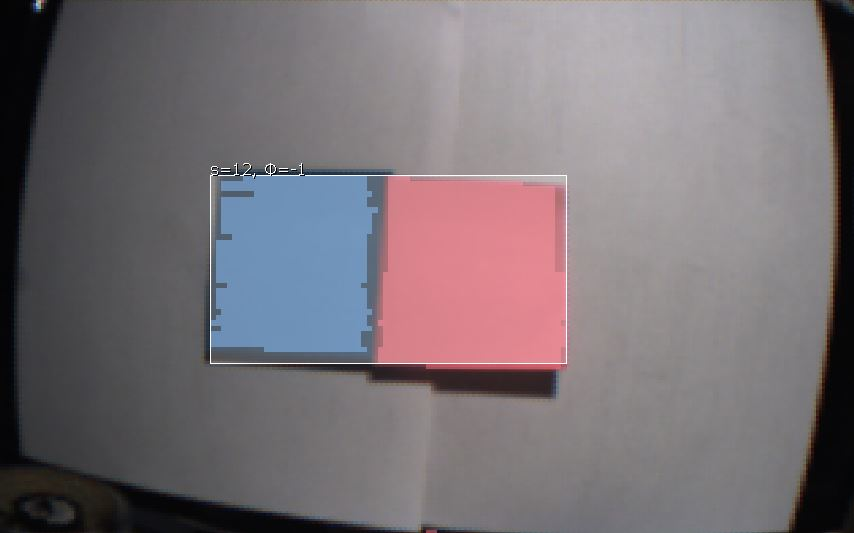
\includegraphics[width = \textwidth]{Bilder/Farbcode_erkannt}
      \par\end{centering}
      \caption{Ein erkannter Farbcode}
      \label{Farbcode_erkannt}
    \end{figure}
    Die Position wird anhand solcher Farbcodes erkannt, im Tischkonzept ist hinterlegt in welcher Reihenfolge der Hexacopter die Farbcodes suchen muss.
    Er fliegt anschließend so lange, bis er über dem aktuellen Farbcode ist, dieser also mittig im Bild ist und sucht darauf den nächsten.


    Die PIXY CMUcam5 XXXXXX % IRGENDWAS MIT X diese länge, y diese länge; %



      \begin{itemize}
        \item \textbf{Überprüfen von Aileron}\\
        Die Überprüfung von Aileron bezieht sich auf die Beschleunigung nach Links und Rechts, was der x-Koordinate entspricht.

        Ziel der Funktion ist es, den Farbcode in die Mitte des Frames zu bekommen. Der Idealzustand befindet sich zwischen 150 und 170.
        Sollte dieser Zustand erreicht werden, bleibt der Wert von Aileron unverändert und der Hexacopter fliegt weiterhin mit einer unveränderten Beschleunigung an der
        x-Koordinate.
        Sollte dies nicht der Fall sein, muss der Wert auf einige Komponenten \textcolor{red}{XXXXX} überprüft werden.
        Wenn der Farbcode zu weit auf der rechten Seite liegt, das bedeutet, wenn der Wert des Mittelpunktes vom Farbobjekt höher als 170 ist,
        muss der Hexacopter nach rechts fliegen, um seine Position zu korrigieren.
        Dabei muss zuerst verglichen werden, ob sich der Hexacopter in die richtige Richtung bewegt. Sollte er in die falsche Richtung
        fliegen, wird der Aileron-Flugparameter gesenkt, dies setzt die Beschleunigung nach Rechts vorraus.
        Wenn die Beschleunigung nach rechts hoch genug ist und die Drohne tatsächlich nach rechts fliegt, wird die Geschwindigkeit überprüft.
        Die Geschwindigkeit wird durch die Differenz der x-Koordinate beider Strukturen herausgefunden. Die Einheit ist in diesem Fall

        \item \textbf{Überprüfen von Elevator}\\
        Position der Farbobjekte (CHECK AILERON \& ELEVATOR)
        Wenn ein Farbobjekt nicht im gewünschten Bereich plaziert ist, muss der Hexacopter weiter nach links oder weiter nach rechts fliegen.
        \item \textbf{Überprüfen von Rudder}\\
        Rotation der Farbojekte (CHECK RUDDER)
        Wenn der Hexacopter über einem Farbobjekt fliegt, soll er kontrollieren, ob der 2-Farbige Code die richtige Rotation hat und sich im richtigen Bereich des Bildschirmes befindet. Wenn diese Informationen richtig sind, darf der Copter zum nächsten Farbobjekt fliegen.
        Durch dieses System könne die genauen Wege vorgegeben werden und können sich durch das gesamte Restaurant verteilen. Durch die Rotation der Codes können auch Kurven eingebaut werden.

        Richtung (CHECK RUDDER)
        Durch die Rotation der Colorcodes, kann der Hexacopter bestimmen, ob er den richtigen Weg und in die richtige Richtung fliegt, wenn er am Weg zurück zur Base ist, muss er den umgekehrten Colorcode verwenden. (Rotation 180Grad)
      \end{itemize}

    \subsubsection{Throttle anhand des Ultraschallsensors}

    Der Hexacopter steht auf einer Landeplattform in seiner Base. Unter ihm ist ein Farbcode, diesen fokusiert er so lange, bis er den nächsten Farbcode trackt. Den zweiten Farbcode kann er erst scannen, wenn er hoch genug fliegt um an der Tischkante vorbei, den nächsten Farbcode zu scannen.
    Beim Starten fliegt er vertikal nach oben, bis er den 2. Farbcode erkennt. Um beim Start nicht abzudriften, beschleunigt er, solange er sich unter einer Höhe von 50cm befindet, mit einer Hohen Änderungsrate. Ab dieser Höhe, beschleunigt er mit einer geringeren Erhöhung der Änderungsrate, bis er die 80cm-Grenze erreicht hat. 
    zwischen 80 und 120cm bleibt die Beschleunigung gleich, das führt jedoch dazu, dass der Hexacopter den oberen Rand von 120 erreichen wird, da er bis jetzt nicht gebremst wird. Sobald er über 120cm kommt, wird die Beschleunigung nach unten hin verändert. Der Hexacopter pendelt also zwischen 80 und 120cm.

    \textbf{P-Regler}\\
    Um Pendelungen entgegenzuwirken gibt es den sogenannten P-Regler.
    % Erklärung P-Regler%

    Nun muss er herausfinden, ob er sich noch über dem Tisch oder schon über dem Boden befindet. Dies stellt er fest, wenn 2 hintereinanderliegende Messungen 50cm von der Vorigen abweichen. Die zweite Messung ist erforderlich, um mögliche Fehlmessungen auszuschließen.

    Wenn er nun über dem Boden fliegt, beträgt seine minimale Höhe bei 180 cm und seine maximale Höhe bei 220 cm.
    Der Hexacopter beschleunigt nach dem selben Prinzip, wie über einem Tisch. Unter 100 cm ändert erhöht er seine Beschläunigung mit einem hohen Wert. Bis 180cm beschleunigt er mit einer niedrigeren Änderungsrate. Zwischen 180 und 220 cm kommt der P-Regler zum Einsatz. Sollte der Hexacopter über 220cm fliegen, wird die Beschleunigung durch eine negative Änderungsrate gesenkt.

    Der Hexacopter fliegt mit diesen Werten, bis er den vorletzten Farbcode erreicht hat. Da die Farbcodes in einem Array abgespeichert werden, ist die Anzahl der darin gespeicherten Farbcodes bekannt. 

    Beim letzten Farbcode angekommen, also dem am Tisch liegenden Farbcode, wird ebenfalls wieder durch die Kontrolle von 2 Werten, die sich um 50cm von der vorigen Messung unterscheiden müssen, analysiert, wann sich der Hexacopter auf dem Tisch befindet. Sobald er sich am Tisch befindet, landet er, indem er die Beschleunigung mit einer negativen Änderungsrate verlangsamt. Dabei muss er sich zwischen einer vom System vorgegebenen Mindest und Maximalgeschwindigkeit befinden. 

    Nach der Landung wird die Routeninformation umgekehrt, die Rotation der Farbcodes muss beim Rückflug um 180 Grad gedreht sein.

    Damit genügend Zeit für das herunternehmen des Cupcakes ist, verweilt der Hexacopter eine halbe Minute am Tisch, bevor er seinen Rückflug antritt.

    \subsubsection{Speichern der alten Daten}
    Die alten Daten werden gespeichert, um die Differenzen von zwei Frames zu errechnen. Der Frame mit Index 0, ist der aktuelle Frame, der Frame mit dem Index 1, der alte. Bei jedem durchlauf, werden die Werte aktualisiert.


    \subsubsection{Ausgabe der Steuersignal}
    Nachdem die Steuersignale berechnet und korrigiert wurden müssen diese an den Hexacopter ausgegeben werden. Dies muss periodisch alle $\SI{20}{\milli\second}$ geschehen.
    Der Flightcontroller erkennt jeweils die einzelnen Impulse und steuert die Rotoren entsprechend an.

    Diese Impulse werden Interrupt-gesteuert ausgegeben, der Interrupt wird von dem Gear-Pin erzeugt welcher gleichzeitig für den Flugmodus verantwortlich ist.

    \lstset{language = c}
    \begin{lstlisting}
interrupt void Isr() {
  if(CCP1IF == 1) {
    CCP1IF = 0;
    T1CONbits.TMR1ON = 0;
    SignalOut();
    NOP();
  }
  if(TMR3GIF == 1) {
    TMR3GIF = 0;
    ModeCheck();
    SignalOut();    /* initial call after remaining break to 20 ms
                     * starts with Aileron (needs to be set in last
                     * case statement, case 0) following delays will
                     * be processed by the previous routine */
    pulsecounter++;
  }
}

void SignalOut(void) {
  switch(pin_out) {
    case 'A': {
      A = 1;
      Delay(a_actors[0].aile);
      pin_out = 'E';
      break;
    }case 'E': {
      A = 0;
      E = 1;
      Delay(a_actors[0].elev);
      pin_out = 'T';
      break;
    }
    \end{lstlisting}
    Die weiteren Signale (Throttle und Rudder) werden auf die gleiche Weise ausgegeben.
    Die Delay-Funktion stellt die Compare-Einehit so ein, dass nach der gewünschten Pulsdauer des Ausgangs ein Interrupt hervorgerufen wird.

%%%%%%%%%%%%%%%%%%%%%%%%%%%%%%%%%%%%%%%%%%%%%%%%%%%%%%%%%%%%%%%%%%%%%%%%%%%%%%%
\section{Objekterkennung}

  \subsection{Technische Planung}

  \subsection{Umsetzung}

  \subsection{Herausforderungen und Lösungen}

%%%%%%%%%%%%%%%%%%%%%%%%%%%%%%%%%%%%%%%%%%%%%%%%%%%%%%%%%%%%%%%%%%%%%%%%%%%%%%%
\section{Sicherheit}

  \subsection{Technische Planung}

  \subsection{Umsetzung}

  \subsection{Herausforderungen und Lösungen}

%%%%%%%%%%%%%%%%%%%%%%%%%%%%%%%%%%%%%%%%%%%%%%%%%%%%%%%%%%%%%%%%%%%%%%%%%%%%%%%
\section{Systemausfall}

  \subsection{Technische Planung}

  \subsection{Umsetzung}

  \subsection{Herausforderungen und Lösungen}
